\documentclass[notes]{beamer}
\usetheme{Madrid}
\usecolortheme{whale}

% Logo and footer setup
\usepackage{graphicx}

% Custom footer
\setbeamertemplate{footline}{
  \leavevmode%
  \hbox{%
  \begin{beamercolorbox}[wd=.1\paperwidth,ht=2.25ex,dp=1ex,center]{date in head/foot}%
    
\includegraphics[height=2ex]{ua_logo.png}
  \end{beamercolorbox}%
  \begin{beamercolorbox}[wd=.8\paperwidth,ht=2.25ex,dp=1ex,center]{title in head/foot}%
    \usebeamerfont{title in head/foot}\insertshorttitle
  \end{beamercolorbox}%
  \begin{beamercolorbox}[wd=.1\paperwidth,ht=2.25ex,dp=1ex,right]{date in head/foot}%
    \usebeamerfont{date in head/foot}\insertframenumber{}/\inserttotalframenumber\hspace*{2ex}
  \end{beamercolorbox}}%
  \vskip0pt%
}

\title{Document Clustering System with Docker}
\subtitle{Technical Mathematics for Big Data}
\author{Oyedotun Oluwasegun Michael (\#123168) \\ Silvia Mastracci (\#123177) \\ Oleksandr Solovei (\#126784)}
\date{January 16, 2025}

\begin{document}

\begin{frame}
    \titlepage
\end{frame}

\begin{frame}{Project Overview}
    \begin{itemize}
        \item Document Clustering System built with microservices
        \item Containerized solution using Docker technology
        \item Key technical components:
        \begin{itemize}
            \item Frontend: React-based UI
            \item Backend: Flask microservices
            \item Search: Elasticsearch engine
            \item Processing: Document analysis system
        \end{itemize}
    \end{itemize}
\end{frame}

\begin{frame}{System Architecture}
    % https://mermaid.ink/img/pako:eNp9VMFu2zAM_RVBvayACmwr0HU-DNgWF-ihQxFvPczJQZWo2IgtBZKctij676MkO3ZWIzpYFPlIPoqUX6kwEmhGVWOeRMWtJ78XK01w_XFgy59NDdqTH9Y84XFNLi6-kV-bWj-X8UuWsAfrgNxb8_yyTo7p67rHjeW7iiyM2IIlud7X1ugWwyVAWClICHqDNg9alkvgwh-OpAC7rwWs53y-39-WNw132yCdRBbArajKtJ1EIlusRZS4d4FrqEyAc8ZO4KMUEo8J3uv7cHOuPZmAyosyxzp8LVxUrmdRS5C1Gy196DnTKOVFn-DBNOWHoyQEVVji-SRZDDMGjD5J9x47TY9yxB4u7RiOfZxOhkAWbgGKuNQHouqmyc74NVwJxZy3ZgvZ2eXj1dcv1_957MKY9XilJGJO4503lm-GDFKAFJ9Oe-wj80MK9Zl_nHWYuMWXwvonQiQo3jV-ak_TFblP1cOMMxwWlvrMhlvtr2YKzwuWetEXdWzDG2dD01jqR18LZbQF2_Ja4jN_DV4r6itoYUUzFAe-dKXfEMo7b4oXLWjmbQeMWtNtKpop3jg8dTvJPSxqjk-7PWh3XP81ZjwjDaR4l34s8f_y9g_PU2Kj?type=png)](https://mermaid.live/edit#pako:eNp9VMFu2zAM_RVBvayACmwr0HU-DNgWF-ihQxFvPczJQZWo2IgtBZKctij676MkO3ZWIzpYFPlIPoqUX6kwEmhGVWOeRMWtJ78XK01w_XFgy59NDdqTH9Y84XFNLi6-kV-bWj-X8UuWsAfrgNxb8_yyTo7p67rHjeW7iiyM2IIlud7X1ugWwyVAWClICHqDNg9alkvgwh-OpAC7rwWs53y-39-WNw132yCdRBbArajKtJ1EIlusRZS4d4FrqEyAc8ZO4KMUEo8J3uv7cHOuPZmAyosyxzp8LVxUrmdRS5C1Gy196DnTKOVFn-DBNOWHoyQEVVji-SRZDDMGjD5J9x47TY9yxB4u7RiOfZxOhkAWbgGKuNQHouqmyc74NVwJxZy3ZgvZ2eXj1dcv1_957MKY9XilJGJO4503lm-GDFKAFJ9Oe-wj80MK9Zl_nHWYuMWXwvonQiQo3jV-ak_TFblP1cOMMxwWlvrMhlvtr2YKzwuWetEXdWzDG2dD01jqR18LZbQF2_Ja4jN_DV4r6itoYUUzFAe-dKXfEMo7b4oXLWjmbQeMWtNtKpop3jg8dTvJPSxqjk-7PWh3XP81ZjwjDaR4l34s8f_y9g_PU2Kj
    
    \vspace*{\fill}
    \begin{center}
        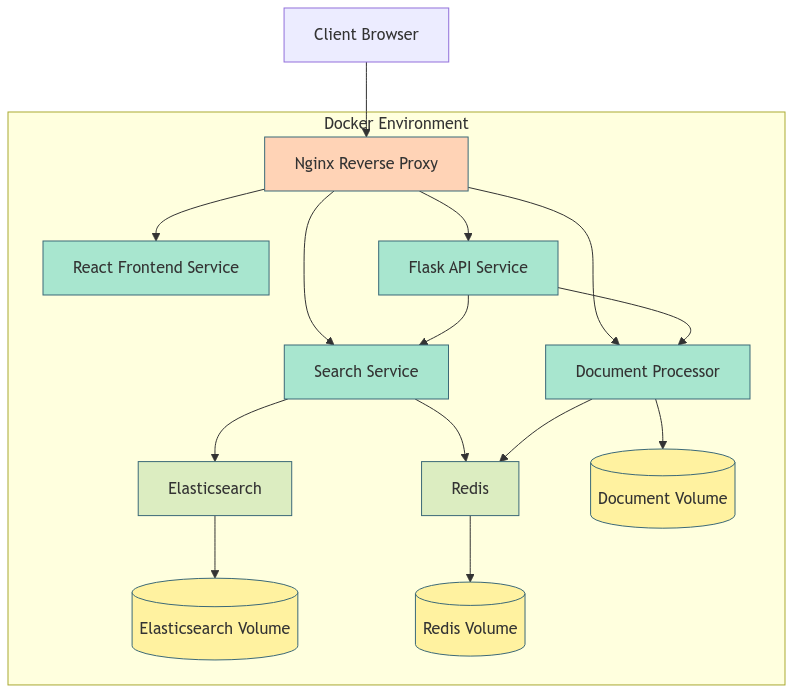
\includegraphics[height=0.84\textheight,keepaspectratio]{systemarch.png}
    \end{center}
    \vspace*{\fill}
\end{frame}


\begin{frame}[fragile]{Docker Compose Configuration}
    \begin{verbatim}
version: '3.8'
services:
  nginx:
    image: nginx:alpine
    ports:
      - "4321:80"
  frontend:
    build: ./frontend
    expose:
      - "3000"
  api:
    build: ./api
    expose:
      - "8000"
  document-processor: (...)
  search: (...)
    \end{verbatim}
\end{frame}


\begin{frame}[fragile]{Running the System}
    Running commands:
    \begin{verbatim}
# Build and start
docker-compose up --build

# Stop services
docker-compose down

# View logs
docker-compose logs -f

# Rebuild specific service
docker-compose build service-name
    \end{verbatim}
\end{frame}

\begin{frame}{Docker Benefits: Development}
    \begin{itemize}
        \item \textbf{Consistent Development Environment}
        \begin{itemize}
            \item Same environment for all team members
            \item "Works on my machine" problem eliminated
            \item Quick onboarding of new developers
        \end{itemize}
        \item \textbf{Isolated Dependencies}
        \begin{itemize}
            \item Each service has its own container
            \item No conflicts between different versions
            \item Easy technology stack updates
        \end{itemize}
        \item \textbf{Rapid Development Cycle}
        \begin{itemize}
            \item Fast container startup
            \item Quick iteration and testing
            \item Easy rollback capabilities
        \end{itemize}
    \end{itemize}
\end{frame}

\begin{frame}{Docker Benefits: Operations}
    \begin{itemize}
        \item \textbf{Resource Efficiency}
        \begin{itemize}
            \item Lightweight container architecture
            \item Optimal resource utilization
            \item Lower infrastructure costs
        \end{itemize}
        \item \textbf{Scalability}
        \begin{itemize}
            \item Easy horizontal scaling
            \item Load balancing support
            \item Dynamic resource allocation
        \end{itemize}
        \item \textbf{Maintenance}
        \begin{itemize}
            \item Simple updates and patches
            \item Minimal downtime
            \item Easy backup and restore
        \end{itemize}
    \end{itemize}
\end{frame}

\begin{frame}{Docker Benefits: Security}
    \begin{itemize}
        \item \textbf{Container Isolation}
        \begin{itemize}
            \item Separate process spaces
            \item Independent network interfaces
            \item Isolated file systems
        \end{itemize}
        \item \textbf{Security Features}
        \begin{itemize}
            \item Resource limitations
            \item Capability restrictions
            \item Network security policies
        \end{itemize}
        \item \textbf{Vulnerability Management}
        \begin{itemize}
            \item Container image scanning
            \item Regular security updates
            \item Immutable infrastructure
        \end{itemize}
    \end{itemize}
\end{frame}

\begin{frame}[fragile]{Project Implementation}
    % Use T (top baseline) alignment for columns themselves
    \begin{columns}[T]
        % Left column with text
        \begin{column}{0.5\textwidth}
            \vspace{1cm}  % Add some top spacing to align with image
            \begin{itemize}
                \item \textbf{Multi-stage builds}
                \begin{itemize}\small
                    \item Optimized image sizes
                    \item Reduced attack surface
                \end{itemize}
                \vspace{0.4cm}
                
                \item \textbf{Docker Compose}
                \begin{itemize}\small
                    \item Service orchestration
                    \item Environment configuration
                    \item Network management
                \end{itemize}
                \vspace{0.4cm}
                
                \item \textbf{Volume Management}
                \begin{itemize}\small
                    \item Persistent data storage
                    \item Efficient data sharing
                \end{itemize}
            \end{itemize}
        \end{column}
        
        % Right column with image
        \begin{column}{0.5\textwidth}
            \centering  % Center the image horizontally
            \vspace{0.5cm}  % Adjust top margin
            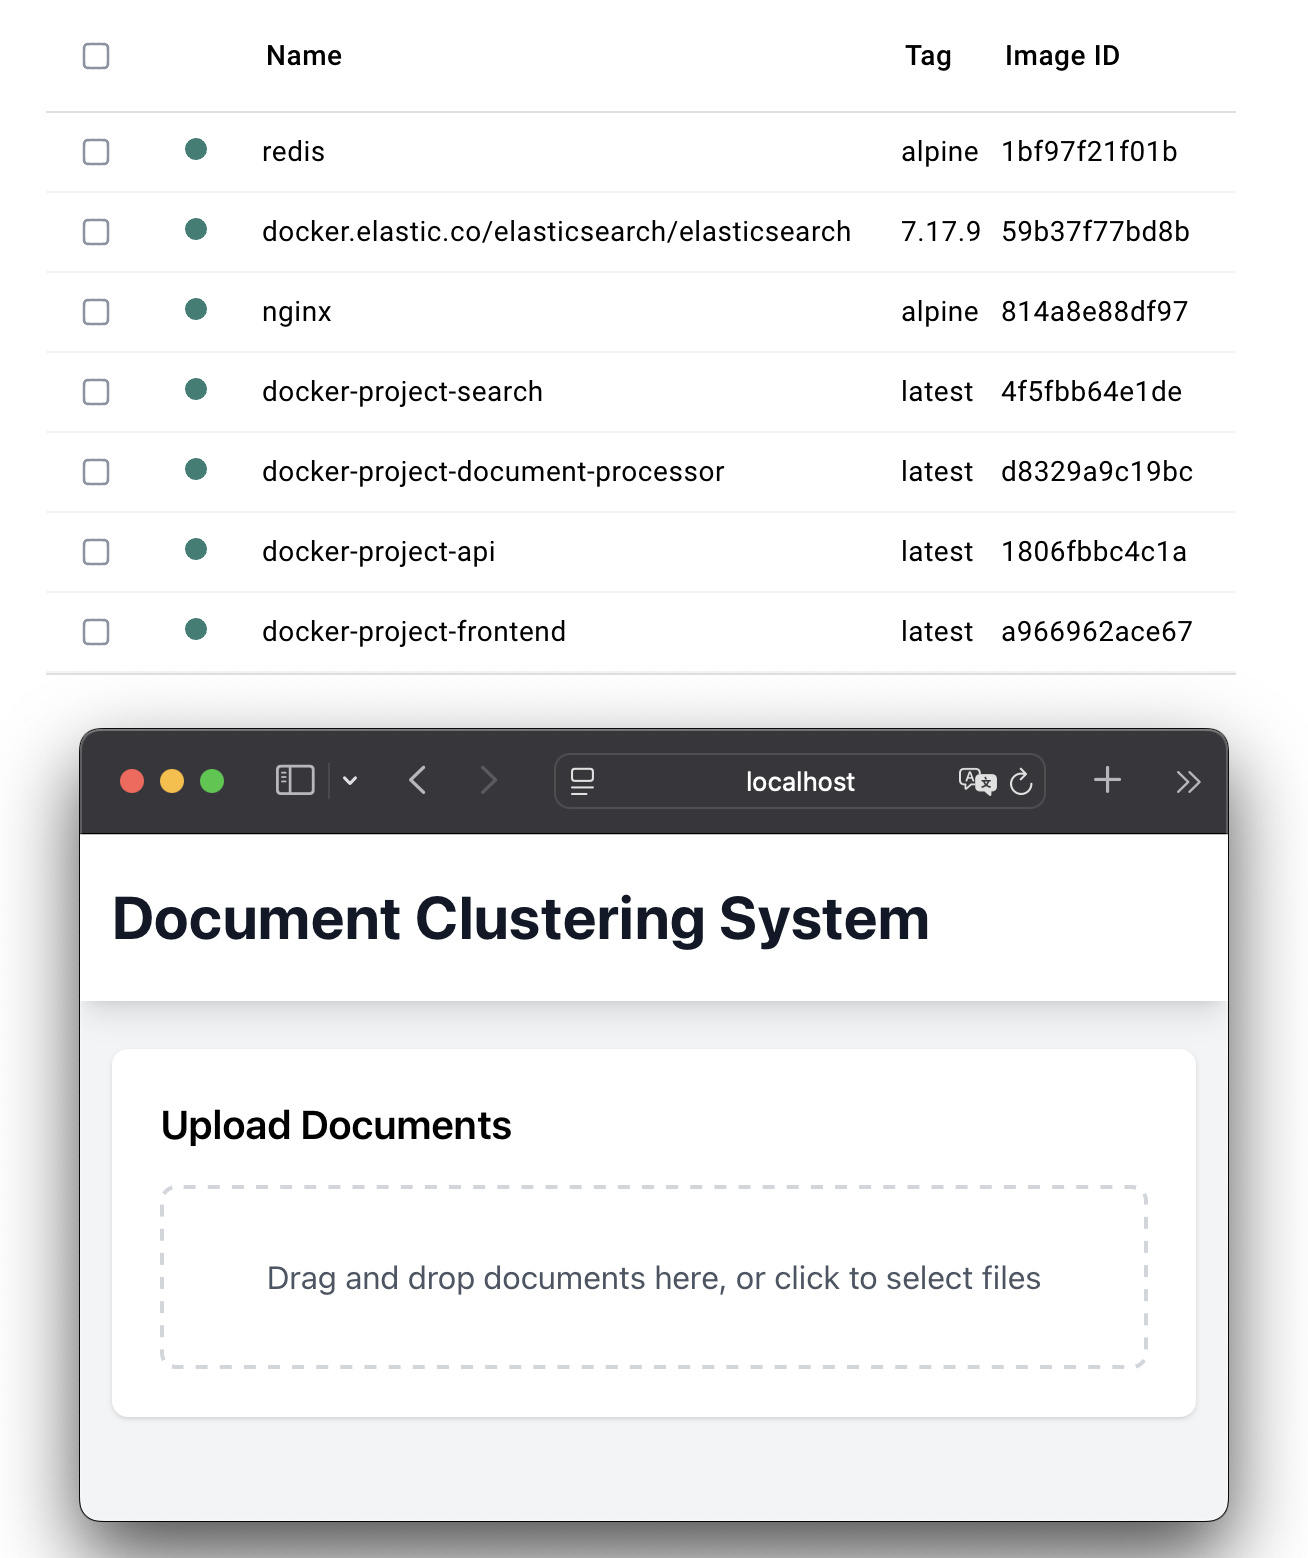
\includegraphics[width=0.95\textwidth,height=0.7\textheight,keepaspectratio]{screenshot.png}
        \end{column}
    \end{columns}
\end{frame}

\begin{frame}{System Features}
    \begin{itemize}
        \item \textbf{Single Port Access}
        \begin{itemize}
            \item All services through one port
            \item Nginx reverse proxy
            \item Simplified deployment
        \end{itemize}
        \item \textbf{Monitoring}
        \begin{itemize}
            \item Health checks
            \item Service discovery
            \item Automated recovery
        \end{itemize}
        \item \textbf{Data Management}
        \begin{itemize}
            \item Elasticsearch integration
            \item Redis caching
            \item Persistent storage
        \end{itemize}
    \end{itemize}
\end{frame}

\begin{frame}{Conclusion}
    \begin{center}
        \Large{Thank You}
        
        \vspace{0.5cm}
        \normalsize{Document Clustering System}\\
        Docker-based Microservices Architecture
        
        \vspace{0.5cm}
        Questions?
    \end{center}
\end{frame}

\end{document}